% Options for packages loaded elsewhere
\PassOptionsToPackage{unicode}{hyperref}
\PassOptionsToPackage{hyphens}{url}
\documentclass[
  11pt,
]{article}
\usepackage{xcolor}
\usepackage[margin=1in]{geometry}
\usepackage{amsmath,amssymb}
\setcounter{secnumdepth}{5}
\usepackage{iftex}
\ifPDFTeX
  \usepackage[T1]{fontenc}
  \usepackage[utf8]{inputenc}
  \usepackage{textcomp} % provide euro and other symbols
\else % if luatex or xetex
  \usepackage{unicode-math} % this also loads fontspec
  \defaultfontfeatures{Scale=MatchLowercase}
  \defaultfontfeatures[\rmfamily]{Ligatures=TeX,Scale=1}
\fi
\usepackage{lmodern}
\ifPDFTeX\else
  % xetex/luatex font selection
\fi
% Use upquote if available, for straight quotes in verbatim environments
\IfFileExists{upquote.sty}{\usepackage{upquote}}{}
\IfFileExists{microtype.sty}{% use microtype if available
  \usepackage[]{microtype}
  \UseMicrotypeSet[protrusion]{basicmath} % disable protrusion for tt fonts
}{}
\makeatletter
\@ifundefined{KOMAClassName}{% if non-KOMA class
  \IfFileExists{parskip.sty}{%
    \usepackage{parskip}
  }{% else
    \setlength{\parindent}{0pt}
    \setlength{\parskip}{6pt plus 2pt minus 1pt}}
}{% if KOMA class
  \KOMAoptions{parskip=half}}
\makeatother
\usepackage{longtable,booktabs,array}
\usepackage{calc} % for calculating minipage widths
% Correct order of tables after \paragraph or \subparagraph
\usepackage{etoolbox}
\makeatletter
\patchcmd\longtable{\par}{\if@noskipsec\mbox{}\fi\par}{}{}
\makeatother
% Allow footnotes in longtable head/foot
\IfFileExists{footnotehyper.sty}{\usepackage{footnotehyper}}{\usepackage{footnote}}
\makesavenoteenv{longtable}
\usepackage{graphicx}
\makeatletter
\newsavebox\pandoc@box
\newcommand*\pandocbounded[1]{% scales image to fit in text height/width
  \sbox\pandoc@box{#1}%
  \Gscale@div\@tempa{\textheight}{\dimexpr\ht\pandoc@box+\dp\pandoc@box\relax}%
  \Gscale@div\@tempb{\linewidth}{\wd\pandoc@box}%
  \ifdim\@tempb\p@<\@tempa\p@\let\@tempa\@tempb\fi% select the smaller of both
  \ifdim\@tempa\p@<\p@\scalebox{\@tempa}{\usebox\pandoc@box}%
  \else\usebox{\pandoc@box}%
  \fi%
}
% Set default figure placement to htbp
\def\fps@figure{htbp}
\makeatother
% definitions for citeproc citations
\NewDocumentCommand\citeproctext{}{}
\NewDocumentCommand\citeproc{mm}{%
  \begingroup\def\citeproctext{#2}\cite{#1}\endgroup}
\makeatletter
 % allow citations to break across lines
 \let\@cite@ofmt\@firstofone
 % avoid brackets around text for \cite:
 \def\@biblabel#1{}
 \def\@cite#1#2{{#1\if@tempswa , #2\fi}}
\makeatother
\newlength{\cslhangindent}
\setlength{\cslhangindent}{1.5em}
\newlength{\csllabelwidth}
\setlength{\csllabelwidth}{3em}
\newenvironment{CSLReferences}[2] % #1 hanging-indent, #2 entry-spacing
 {\begin{list}{}{%
  \setlength{\itemindent}{0pt}
  \setlength{\leftmargin}{0pt}
  \setlength{\parsep}{0pt}
  % turn on hanging indent if param 1 is 1
  \ifodd #1
   \setlength{\leftmargin}{\cslhangindent}
   \setlength{\itemindent}{-1\cslhangindent}
  \fi
  % set entry spacing
  \setlength{\itemsep}{#2\baselineskip}}}
 {\end{list}}
\usepackage{calc}
\newcommand{\CSLBlock}[1]{\hfill\break\parbox[t]{\linewidth}{\strut\ignorespaces#1\strut}}
\newcommand{\CSLLeftMargin}[1]{\parbox[t]{\csllabelwidth}{\strut#1\strut}}
\newcommand{\CSLRightInline}[1]{\parbox[t]{\linewidth - \csllabelwidth}{\strut#1\strut}}
\newcommand{\CSLIndent}[1]{\hspace{\cslhangindent}#1}
\setlength{\emergencystretch}{3em} % prevent overfull lines
\providecommand{\tightlist}{%
  \setlength{\itemsep}{0pt}\setlength{\parskip}{0pt}}
\usepackage{fancyhdr}
\pagestyle{fancy}
\fancyhead[L]{\textit{Forensic Modelling of Blood Alcohol Evidence}}
\fancyhead[R]{\leftmark}
\fancyfoot[C]{\thepage}
\usepackage{setspace}
\onehalfspacing
\usepackage{titling}
\pretitle{\begin{center}\LARGE\bfseries}
\posttitle{\end{center}\vspace{1em}}
\usepackage{caption}
\captionsetup[figure]{labelfont=bf,textfont=it}
\captionsetup[table]{labelfont=bf}
\usepackage{titlesec}
\newcommand{\sectionbreak}{\clearpage}
\renewcommand{\citeproc}[2]{%
  \hyperref[#1]{\textcolor{blue}{#2}}%
}

\let\oldbibitem\bibitem
\renewcommand{\bibitem}[2][]{%
  \oldbibitem[#1]{#2}%
  \phantomsection\label{#2}%
} 

\preauthor{\begin{center}\large}
\postauthor{\end{center}}
\usepackage{booktabs}
\usepackage{longtable}
\usepackage{array}
\usepackage{multirow}
\usepackage{wrapfig}
\usepackage{float}
\usepackage{colortbl}
\usepackage{pdflscape}
\usepackage{tabu}
\usepackage{threeparttable}
\usepackage{threeparttablex}
\usepackage[normalem]{ulem}
\usepackage{makecell}
\usepackage{xcolor}
\usepackage{bookmark}
\IfFileExists{xurl.sty}{\usepackage{xurl}}{} % add URL line breaks if available
\urlstyle{same}
\hypersetup{
  pdftitle={Forensic Modelling of Blood Alcohol Evidence},
  hidelinks,
  pdfcreator={LaTeX via pandoc}}

\title{Forensic Modelling of Blood Alcohol Evidence}
\author{Group 13\textbackslash\textbackslash{} Du Shi, Kunning Zhang,
Yixuan Yin\textbackslash\textbackslash{} Total words: 3668}
\date{November 19, 2025}

\begin{document}
\maketitle

{
\setcounter{tocdepth}{3}
\tableofcontents
}
\section{Executive Summary}\label{executive-summary}

In the UK it is a criminal offence to drive a motor vehicle with a blood
or breath alcohol concentration above the prescribed limit. When a
person is arrested for driving under the influence of alcohol it is not
usually possible to perform an accurate test of the level of alcohol in
the blood or breath immediately. Breath tests can be used as an initial
screening tool at the scene, but these are not sufficiently accurate for
prosecution. Instead, people are taken to a police station or hospital,
where the test can be carried out using proper laboratory protocols. As
the body clears alcohol from the blood through time this means that if
the individual was over the limit, the measured blood alcohol
concentration (BAC) will be lower at the time of measurement than it was
when the person was driving a motor vehicle. To deal with this
situation, If the BAC after time \(t\) (hours) is measured as \(C_t\)
(g/kg), the BAC at time \(0\) is estimated as \(C_0 = C_t - βt\), where
\(\beta\) (\(g/kg/h\)) is BAC elimination rate.

The key point is how to find a precise \(\beta\) to estimate \(C_0\).
Forensic scientists currently use \(2.5\%\) percentile of \(\beta\)
distribution constructing from samples as the estimated \(\beta\) value
for every individuals. This method is obviously not rigorous for the
courts.

In this report, we introduce a Bayesian Regression Model (BRM) with
considering the heterogeneity between individuals, the model gives a
posterior distribution of \(\hat{\beta}\) by using both samples and
prior knowledge. Then we use Markov Chain Monte Carlo (MCMC) to simulate
\(12000\) \(\beta\) draws from posterior distribution and find out the
probability of the person's BAC over limit while driving.

In real world, \(\beta\) estimation is quite difficult, it depends on
the individuals' liver condition, drinking habits, genetic, diet, etc.
As we don't have corresponding data, variation of \(\beta\) is mainly
explained by gender, but we still find some useful variables like
`weight' and `drinking time'.

When it is too late to use a blood or breath test and the only
information available is eyewitness testimony of the quantity of alcohol
consumed. We have to use Widmark's equation:
\[C_t = \frac{A}{Weight \times V_d} - \beta t\]

where \(A\) is Amount of Alcohol Consumed (g), \(V_d\) is the volume of
distribution that need to be found.

Forensic scientists use the same method again to estimate \(V_d\)
separately with \(\beta\). But \(V_d\) and \(\beta\) are not
independent, so the method is also unavailable. To improve it, we build
a joint Bayesian regression model, which can simulate them together to
solve with the correlation. Then again after simulation, each \(C_t\) is
calculated by each pair of \(\beta\) and \(V_d\), so expert witness can
still find a probability of \(C_t\) exceeding the limit.

Results will be provided in format of table \(5\).

\section{Data Description}\label{data-description}

\(\beta\) true values are converted to positive to convenient
calculation.

It is important to normalized all numerical variables. Centering the
covariates can reduce autocorrelation \(\rho_k\) of lag \(k\) which is
defined as:

\[\rho_k = \frac{Cov(\theta^i, \theta^{i+k})}{\theta^2}.\]

`\(\rho_k\)' is an important indicator to show the performance of a BRM
model, it measures how similar the sample at position \(i\) is to the
sample at position \(i+k\). Since MCMC is a random walk process,
\(\theta_i\) should be similar to \(\theta_{i+1}\), less similar to
\(\theta_{i+2}\), independent with \(\theta_{i+k}\) for large \(k\). So
if \(\rho_k\) is large means the chains hardly move, can't converge.

To make it more clear, we will use Effective Sample Size (ESS) to
explain:

\[ n_{\text{eff}} = \frac{n}{1 + 2 \sum_{k=1}^{\infty}\rho_k}.\]

`\(n_{\text{eff}}\)' is large means the MCMC method converge faster (for
example \(n_{\text{eff}} = 10000\) means the number of independent
samples is \(10000\) out of \(16000\)). Larger \(n_{\text{eff}}\) in
same number of iterations means smaller variance of estimated
exoectation since:

\[\mathrm{V}(\hat{E}(\beta)) \approx \frac{\sigma^2}{n_{\text{eff}}}.\]

That's basically why we standardized variables, the statistic ESS will
appear in the modeling results.

Also Since \(\beta\) is a small value, the coefficients of large value
variables are pretty small, near 0, which will make \(\beta\) estimation
worse, so normalization for variables is necessary.

Then we prefer to \(\beta\) to \(\log(\beta)\) since the original
\(\beta\) distribution has heavy tail. As shown in figure 1,
\(\text{log} \beta\) forms a better distribution shape. After simulation
we take exponential of the results.

\begin{figure}
\centering
\pandocbounded{\includegraphics[keepaspectratio]{P2_files/figure-latex/unnamed-chunk-2-1.pdf}}
\caption{log(beta) distribution.}
\end{figure}

Since \(\beta\) is a constant rate, measured when the BAC curve reaches
peak and starts to decrease, so variables like AAC and Maximum BAC will
not be used, since they are correlated with the value of BAC, not BAC
elimination rate.

From the dataset, most data comes from age smaller than \(30\), so even
though age is a sufficient variable for \(\beta\) the model can't really
recognize it. Research shows that age doesn't really matter unless the
subject has age-related liver disease, but because of moral and ethical,
we don't find much research of alcohol test on elderly person with liver
disease.

`BAC Peak time' is converted to hours.

\section{Bayesian regression model}\label{bayesian-regression-model}

\subsection{Advantages and disadvantages of exists
method}\label{advantages-and-disadvantages-of-exists-method}

Although the forensic scientists' method is easy to calculate and
conservative enough, but:

\begin{itemize}
\tightlist
\item
  The courts will be forced to make decisions under estimated
  \(\hat{\beta}\) if we only give a single expectation value, since the
  calculated \(C_0\) is either over or under the legal limit. Our job is
  helping courts make decisions.
\item
  Differences between individuals are ignored, for example weight and
  sex, which may affect \(\beta\).
\item
  \(\beta\) value at \(2.5\%\) is over conservative and most
  uncertainties are hiding.
\end{itemize}

So we don't suggest it.

\subsection{Reasons for BRM and
advantage}\label{reasons-for-brm-and-advantage}

Comparing with fitting linear regression model for \(\beta_i\), which
can be expressed as:

\[\hat{\beta}_{j} = \hat{\gamma}X_j + \varepsilon_{\beta}, \quad \varepsilon_{\beta} \sim N(0, \sigma_{\beta}^2)\]

and giving a exact value of \(\hat{\beta_j}\) under \(\varepsilon\) for
\(j_{th}\) individuals, BRM can model uncertainty of each coefficient
\(\hat{\gamma}\) and \(\varepsilon\). We provide priors and sample
likelihoods for all \(\hat{\gamma}\) and \(\varepsilon\) , BRM will
apply bayesian rule to each and output simulation results of each
coefficients, not only for \(\hat{\beta}\). \(\hat{\beta}\)s are
calculated from simulation results of \(\hat{\gamma_j}\), which is:

\[\hat{\beta}_{i,j} = \hat{\gamma}_{i}X_j + \hat{\varepsilon}_{{\beta},i}, \quad \hat{\varepsilon}_{\beta,i} \sim N(0, \hat{\sigma}_{\beta}^2)\]

where \(i\) is \(i_{th}\) simulation draws.

Since we have log-transformed \(\beta\) data points, we will take
exponential of \(\hat{\beta}_{i,j}\).

\subsection{How BRM works}\label{how-brm-works}

The principle theorem behind BRM is Bayes' Rule:

\[p(\theta \mid \text{data}) = \frac{p(\text{data} \mid \theta) \, p(\theta)}{p(\text{data})}.\]

The \(\theta\) in the equation is the \(\gamma\)s and \(\varepsilon\).
For most real models, we can't compute this posterior
\(p(\theta \mid \text{data})\) analytically. Markov Chain Monte Carlo
(MCMC) helps us draw samples from it, which we can then summarize. BRM
uses Hamiltonian Monte Carlo (One of MCMC), which is better than
standard MCMC (like Metropolis-Hastings) since it is faster and cost
less.

After setting priors for \(\gamma\)s and \(\varepsilon\), we need
specify a family for \(\beta\) as the the likelihood of the observed
data. In our sample, we have already taken \(\log(\beta)\), so it is
better to use the most common normal distribution likelihood, it is
normal and can express \(\beta\) values good without restrict samples'
shape.

Also for the MCMC simulation method, we set \(4\) chains, each chains
\(4000\) draws with \(1000\) burn-in draws. Since MCMC is a random walk
method through parameter space. One chain is a single run of the MCMC
algorithm that generates a sequence of samples, so we need more chains
to check the convergence and ensure that all chains convergent to same
mode.

For \(1000\) burn-in draws, since MCMC starts from an initial value
which often far from the true posterior region, so the chains need some
steps to walk to the correct trace. As figure 2 shows, it is an example
of the MCMC process of coefficient of `female' when using \(4\) chains,
\(100\) draws. Clearly that if we keep the first \(25\) draws, the
results will be affected.

\begin{figure}
\centering
\pandocbounded{\includegraphics[keepaspectratio]{P2_files/figure-latex/unnamed-chunk-3-1.pdf}}
\caption{MCMC Simulations Traceplot.}
\end{figure}

\subsection{Model Selection}\label{model-selection}

\subsubsection{Key Variables}\label{key-variables}

We remove the intercept and use gender (male and female) to be the two
baselines. Since \(\beta\) for male and female are in different range.

\begin{itemize}
\item
  Gender: Female's BAC elimination rate is larger than male on average
  (figure 3), it is explained by liver weight represents a greater
  fraction of lean body mass in the female gender.
  \citeproc{ref-kwo1998gender}{{[}1{]}}
\item
  Drinking time: If the person keep drinking after BAC reaches peak, the
  measured \(\beta\) will be smaller since \(\beta\) is measured
  starting at BAC peak time till the end, there will be fluctuations on
  the BAC plots. We will use total drinking time as the indicator.
\item
  Weight and Height: Basically higher weight often leads lager size of
  liver and larger amount of total body water. Height also affect the
  amount of total body water. \citeproc{ref-maskell2020total}{{[}2{]}}
\end{itemize}

\begin{figure}
\centering
\pandocbounded{\includegraphics[keepaspectratio]{P2_files/figure-latex/Figure-1.pdf}}
\caption{Box plot of beta respect to gender.}
\end{figure}

So the final regression model is:

\[\hat{\beta}_{i,j} = \hat{\gamma}_{1,i}\,\text{female}_j
+ \hat{\gamma}_{2,i}\,\text{male}_j
+ \hat{\gamma}_{3,i}\,\text{weight}_j
+ \hat{\gamma}_{4,i}\,\text{height}_j + \varepsilon_{\beta,i} , \quad \varepsilon_{\beta,i} \sim N(0, \sigma_{\beta}^2).\]

\subsubsection{Priors}\label{priors}

Before fitting the Bayesian regression model, appropriate priors need to
be specified for all regression coefficients and the residual standard
deviation. We use weakly informative priors, which have small effects on
the posterior. The selected priors are summarized as follows:

\begin{longtable}[]{@{}ll@{}}
\caption{Weakly informative priors}\tabularnewline
\toprule\noalign{}
& Prior \\
\midrule\noalign{}
\endfirsthead
\toprule\noalign{}
& Prior \\
\midrule\noalign{}
\endhead
\bottomrule\noalign{}
\endlastfoot
Regression coefficient for male & Normal(0, 2) \\
Regression coefficient for female & Normal(0, 2) \\
Regression coefficients (others) & Normal(0, 0.5) \\
Residual SD & Exponential(1) \\
\end{longtable}

We do not expect \(\beta\) to have a linear relationship with the
variables, so zero-mean normal priors are appropriate. We consider
gender to be the baseline factor influencing alcohol elimination rates,
so we set relatively wide priors Normal(0, 2) for the sex coefficients,
allowing their effects to vary within a reasonable range. For other
standardized variables, since their impacts are considered relatively
small, we used more shrinkage weakly informative priors Normal(0, 0.5)
to prevent unreasonably large effects. The residual standard deviation
is given an Exponential(\(1\)) prior, which is a commonly used positive
weakly informative prior that can avoid unreasonably high noise.

If future research involves different populations, larger sample sizes,
or additional biological information, the prior distributions can be
adjusted accordingly to ensure they are applicable to any new datasets.

\subsection{Model Results}\label{model-results}

\subsubsection{Fitting result}\label{fitting-result}

After \(4000\) iterations in \(4\) chains, Table \(2\) gives the
posterior summary. `Rhat' compares within-chain variance and
between-chain variance, all less than \(1.01\) means chains are
well‐mixed.

\begin{longtable}[]{@{}
  >{\raggedright\arraybackslash}p{(\linewidth - 14\tabcolsep) * \real{0.1974}}
  >{\raggedleft\arraybackslash}p{(\linewidth - 14\tabcolsep) * \real{0.1184}}
  >{\raggedleft\arraybackslash}p{(\linewidth - 14\tabcolsep) * \real{0.1316}}
  >{\raggedleft\arraybackslash}p{(\linewidth - 14\tabcolsep) * \real{0.1184}}
  >{\raggedleft\arraybackslash}p{(\linewidth - 14\tabcolsep) * \real{0.1184}}
  >{\raggedleft\arraybackslash}p{(\linewidth - 14\tabcolsep) * \real{0.0658}}
  >{\raggedleft\arraybackslash}p{(\linewidth - 14\tabcolsep) * \real{0.1316}}
  >{\raggedleft\arraybackslash}p{(\linewidth - 14\tabcolsep) * \real{0.1184}}@{}}
\caption{Posterior Summary from BRM}\tabularnewline
\toprule\noalign{}
\begin{minipage}[b]{\linewidth}\raggedright
\end{minipage} & \begin{minipage}[b]{\linewidth}\raggedleft
Estimate
\end{minipage} & \begin{minipage}[b]{\linewidth}\raggedleft
Est.Error
\end{minipage} & \begin{minipage}[b]{\linewidth}\raggedleft
l-95\% CI
\end{minipage} & \begin{minipage}[b]{\linewidth}\raggedleft
u-95\% CI
\end{minipage} & \begin{minipage}[b]{\linewidth}\raggedleft
Rhat
\end{minipage} & \begin{minipage}[b]{\linewidth}\raggedleft
Bulk\_ESS
\end{minipage} & \begin{minipage}[b]{\linewidth}\raggedleft
Tail\_ESS
\end{minipage} \\
\midrule\noalign{}
\endfirsthead
\toprule\noalign{}
\begin{minipage}[b]{\linewidth}\raggedright
\end{minipage} & \begin{minipage}[b]{\linewidth}\raggedleft
Estimate
\end{minipage} & \begin{minipage}[b]{\linewidth}\raggedleft
Est.Error
\end{minipage} & \begin{minipage}[b]{\linewidth}\raggedleft
l-95\% CI
\end{minipage} & \begin{minipage}[b]{\linewidth}\raggedleft
u-95\% CI
\end{minipage} & \begin{minipage}[b]{\linewidth}\raggedleft
Rhat
\end{minipage} & \begin{minipage}[b]{\linewidth}\raggedleft
Bulk\_ESS
\end{minipage} & \begin{minipage}[b]{\linewidth}\raggedleft
Tail\_ESS
\end{minipage} \\
\midrule\noalign{}
\endhead
\bottomrule\noalign{}
\endlastfoot
sexfemale & -1.673 & 0.034 & -1.740 & -1.606 & 1 & 8576.353 &
8334.303 \\
sexmale & -1.730 & 0.024 & -1.778 & -1.684 & 1 & 8742.778 & 8309.203 \\
weight\_s & -0.008 & 0.024 & -0.054 & 0.038 & 1 & 8392.999 & 8129.812 \\
height\_s & -0.045 & 0.025 & -0.094 & 0.003 & 1 & 7596.179 & 8023.806 \\
drinkingtime\_s & -0.041 & 0.016 & -0.073 & -0.010 & 1 & 11330.326 &
8349.984 \\
\end{longtable}

Figure 4 shows posterior results for each variables' coefficients, all
coefficients show good normal patterns since all chains have converged
and warm-up length is enough. Since the \(\beta\) is log-transformed,
the value of `b\_sexfemale' and `b\_sexmale' is not typical value of
\(\beta\) like \(0.19\) when other coefficients are all near zero. Also
\(\sigma\) value is estimated under log-transformed \(\beta\).

\begin{figure}
\centering
\pandocbounded{\includegraphics[keepaspectratio]{P2_files/figure-latex/unnamed-chunk-6-1.pdf}}
\caption{Posterioe density of 4 chains for all coefficients.}
\end{figure}

Figure 5 shows the trace plots for all variable coefficients, it can be
seen that all \(4\) chains mix well and all values are picking after
convergent.

\begin{figure}
\centering
\pandocbounded{\includegraphics[keepaspectratio]{P2_files/figure-latex/unnamed-chunk-7-1.pdf}}
\caption{Traceplot of all coefficients and variance sigma.}
\end{figure}

\subsubsection{PPC Density}\label{ppc-density}

Figure 6 is the Posterior Predictive Check (PPC) density plot comparing
with true value of \(\beta\) (Here we have taken exponential of both
true value and predicted value). Notice that predicted posterior
distribution matches \(\beta\) sample distribution pretty well, which
get the mean, spread, skew both right even at right tail.

\begin{figure}
\centering
\pandocbounded{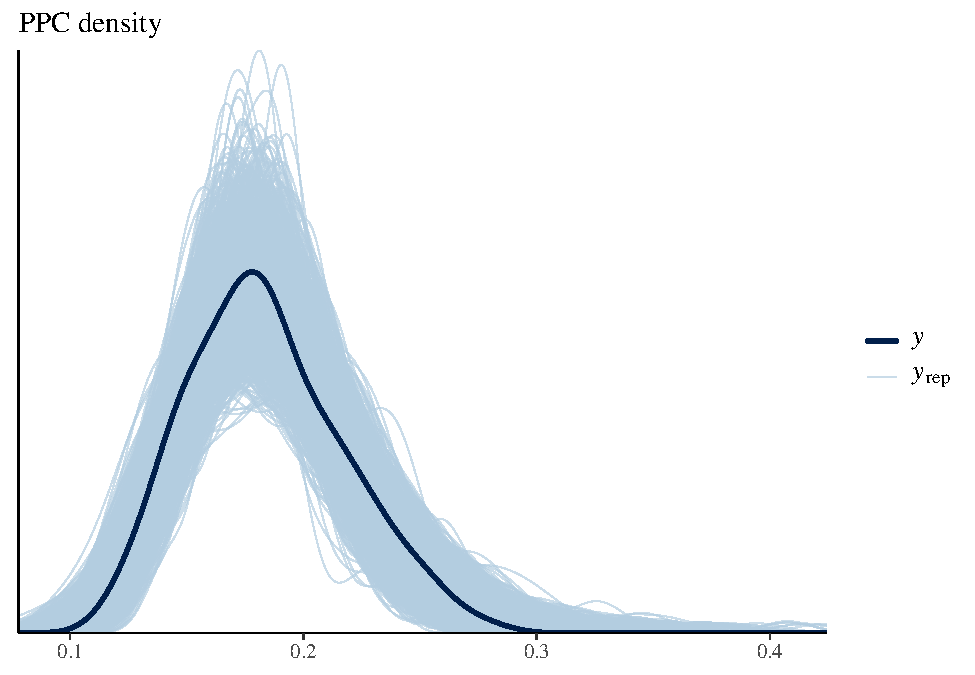
\includegraphics[keepaspectratio]{P2_files/figure-latex/unnamed-chunk-8-1.pdf}}
\caption{PPC density of 2000 predict results from posterior.}
\end{figure}

\subsection{Model Testing}\label{model-testing}

We take all \(12000\) (\(16000\) iterations - \(4000\) warm-up) number
of draws from the posterior distribution.

\subsubsection{LOO-PIT QQ plot}\label{loo-pit-qq-plot}

The Leave-One-Out Probability Integral Transform Quantile-Quantile plot
(LOO-PIT QQ plot) can check if the predictions calibrated correctly and
if the predictive distributions biased, which is defined as:

\[ \mathrm{LOO\text{-}PIT}_i = P(\tilde{y}_i \le y_i |y_{-i}) .\]

Here we still use Monte Carlo method to simulate it, as:

\[
\mathrm{LOO\text{-}PIT}_i
= \frac{1}{S} \sum_{s=1}^{S} 
\mathbf{1}\!\left( \tilde{y}_{i,-i}^{(s)} \le y_i \right)
\]

where \(S\) is the number of posterior draws.

We will use it to check if our posterior is under or over dispersion,
the good model's PIT plot should be flat over \(Uniform(0,1)\). For our
model, the LOO-PIT QQ plot (Figure 7) is flat everywhere except
probability near 0.55 and 0.8, which are acceptable by the randomness of
MCMC method. A U-shape (points over dot line at two tails) in PIT plots
means overestimates variance, it doesn't appear in our plot gives
evidence of our choices on variables and likelihood family.

\begin{figure}
\centering
\pandocbounded{\includegraphics[keepaspectratio]{P2_files/figure-latex/unnamed-chunk-9-1.pdf}}
\caption{LOO-PIT QQ plot}
\end{figure}

\subsubsection{Coverage rate and Errors}\label{coverage-rate-and-errors}

Table 3 shows the coverage rate of \(95\%\) and \(50\%\) predicted
intervals, which means \(98\) and \(51\) individuals' real \(\beta\)
value is inside the intervals. The MAE and RMSE are both relatively
small.

\begin{longtable}[]{@{}lr@{}}
\caption{Testing table}\tabularnewline
\toprule\noalign{}
Metric & Value \\
\midrule\noalign{}
\endfirsthead
\toprule\noalign{}
Metric & Value \\
\midrule\noalign{}
\endhead
\bottomrule\noalign{}
\endlastfoot
95\% predictive interval coverage & 0.980 \\
50\% predictive interval coverage & 0.510 \\
Mean Absolute Error & 0.023 \\
Root Mean Square Error & 0.028 \\
\end{longtable}

\subsubsection{Cross-Validation}\label{cross-validation}

We do two kinds of Cross-Validation: LOO and Kfold (table \(4\)). The
two methods show similar results means the model is stable and the \(p\)
value is near the number of variables (\(5\)) shows the model is not
over-fitting.

\begin{longtable}[t]{lrrrrrr}
\caption{\label{tab:unnamed-chunk-1}Cross-validation Comparison (LOO vs 10-fold)}\\
\toprule
Method & elpd & elpd\_SE & p & p\_SE & IC & IC\_SE\\
\midrule
LOO & 38.672 & 6.321 & 5.636 & 0.857 & -77.344 & 12.643\\
K-fold & 38.648 & 6.156 & 5.660 & 0.894 & -77.296 & 12.312\\
\bottomrule
\end{longtable}

\section{Example}\label{example}

Now we will apply our model on an individual example: A \(70\) year old
female (weight: \(70\)kg, height: \(160\)cm) is arrested after being
stopped by the police while driving. She provides a blood sample to the
police \(2\) hours after her arrest which gives a reading of Ct =
\(0.15\)g/kg. The legal limit is x = \(0.47\)g/kg.

Since there is no `drinking time' data here, we will use a simplified
model with only `sex', `height', `weight' variables. We have
standardized height and weight by using sample's mean and variance.

As figure 8 shows, this is the posterior density of \(C_0\) calculated
by presicted posterior density of \(\hat{\beta}\) the dot line is the
legal limit \(C_0 = 0.47\), it can be seen that most density is larger
than \(0.47\), so obviously the 70 year old female is over the drink
driving limit.

\begin{figure}
\centering
\pandocbounded{\includegraphics[keepaspectratio]{P2_files/figure-latex/unnamed-chunk-12-1.pdf}}
\caption{Posterior Predictive Distribution of C\_0 with limit C\_0 =
0.47 (dot line).}
\end{figure}

To make the result clear, it is better to give Table 5 to the courts and
illustrate:

\begin{center}
There is $91.5\%$ probability that the 70 year old female is over the drink driving limit, with both mean, median and mode value over the limit.
\end{center}

The results also show that the original method is not reasonable since
\(2.5\%\) percentile is over-conservative even in this case.

\begin{longtable}[]{@{}lr@{}}
\caption{Example C\_0 results}\tabularnewline
\toprule\noalign{}
Statistic & Value \\
\midrule\noalign{}
\endfirsthead
\toprule\noalign{}
Statistic & Value \\
\midrule\noalign{}
\endhead
\bottomrule\noalign{}
\endlastfoot
Mean & 0.559 \\
Median & 0.553 \\
Mode & 0.538 \\
2.5\% & 0.438 \\
25\% & 0.509 \\
75\% & 0.603 \\
97.5\% & 0.713 \\
P(C\_0 \textgreater{} 0.47) & 0.911 \\
\end{longtable}

\section{\texorpdfstring{Widmark's Equation and
\(V_d\)}{Widmark's Equation and V\_d}}\label{widmarks-equation-and-v_d}

When it is too late to use a blood or breath test and the only
information available is eyewitness testimony of the quantity of alcohol
consumed. We have to use Widmark's equation:
\[C_t = \frac{A}{Weight \times V_d} - \beta t.\] Since there are many
versions of Widmark's equation, it can also write as:
\[C_t = \frac{F \times A}{Weight \times \rho} - \beta t \] where

\[
\rho = \frac{TBW}{\textit{weight} \times F_{\mathrm{water}}}
\] is known as Widmark's rho factor.

\(F\) is the fraction of the dose that reaches the systemic circulation,
\(F_{\text{water}}\) is know as the water content of the blood sample,
TBW is Total Body Water.

We assume that all different part between two equations are included in
\(V_d\). The unit of \(C_t\) is g/kg in our dataset, the unit of the
first term of \(C_t\) equation is g/L, but it is not a problem since the
density of water is \(1\), we just ignore the \(1\).

\subsection{\texorpdfstring{\(V_d\), TBW and
\(\rho\)}{V\_d, TBW and \textbackslash rho}}\label{v_d-tbw-and-rho}

All information in this part are from `Total body water is the preferred
method to use in forensic blood-alcohol calculations rather than
ethanol's volume of distribution'{[}2{]}.

TBW is calculated by:

\[
\mathrm{TBW}_{\text{Men}}(\mathrm{L}) 
= 2.447 - (0.09516 \times \text{age}) 
    + (0.1074 \times \text{height}) 
    + (0.3362 \times \text{weight})
\]

\[
\mathrm{TBW}_{\text{Women}}(\mathrm{L}) 
= -2.097 
    + (0.1069 \times \text{height}) 
    + (0.2466 \times \text{weight}).
\]

Now subbing the \(\rho\) expression in the \(C_t\) equation, and
comparing with our equation, \(V_d\) is actually calculated by:
\[V_d = \frac{\text{TBW}}{\text{weight}} \times \frac{1}{F_{\text{water}}} \times \frac{1}{F} = \eta \times \frac{\text{TBW}}{\text{weight}}\]
and we need to estimate \(\eta\) value since TBW is a value that can be
determined in our dataset. we will use:

\[\hat{V_d}_{i,j} = \hat{\eta}_{1,i} ( \frac{\text{TBW}}{\text{weight}}_\text{male})_j + \hat{\eta}_{2.i} ( \frac{\text{TBW}}{\text{weight}}_\text{female})_j + \hat{\varepsilon}_{{V_d},{i}}, \quad \hat{\varepsilon}_{{V_d},{i}} \sim N(0, \hat{\sigma}_{V_d}^2)\]
to estimate \(\hat{V_d}\) where \(i\) is the \(i_{th}\) iterations (we
will again use BRM, but as a joint model with \(\beta\) to deal with the
correlation, we will explain it in next part.), \(j\) is the \(j_{th}\)
individuals, \(\eta\) is the coefficients that need to be predicted.

\subsection{\texorpdfstring{Correlations between \(\beta\) and
\(V_d\)}{Correlations between \textbackslash beta and V\_d}}\label{correlations-between-beta-and-v_d}

To show that the correlation can't be ignored, figure 9 gives the
correlations between true \(\beta\) and \(V_d\) is \(-0.415\), which is
relatively big.

\begin{figure}
\centering
\pandocbounded{\includegraphics[keepaspectratio]{P2_files/figure-latex/unnamed-chunk-14-1.pdf}}
\caption{Correlation plot betweem V\_d and Beta}
\end{figure}

\section{\texorpdfstring{Joint Bayesian regression model for \(\beta\)
and
\(V_d\)}{Joint Bayesian regression model for \textbackslash beta and V\_d}}\label{joint-bayesian-regression-model-for-beta-and-v_d}

\subsection{\texorpdfstring{Advantages and disadvantages for exists
method for
\(V_d\)}{Advantages and disadvantages for exists method for V\_d}}\label{advantages-and-disadvantages-for-exists-method-for-v_d}

The exists method is easy to calculate. But as we showed before, the
correlation between \(\beta\) and \(V_d\) is relatively large and can't
be ignored, especially for the courts since we need the calculated
\(C_t\) as precise as possible.

\subsection{\texorpdfstring{Overview of
\(V_d\)}{Overview of V\_d}}\label{overview-of-v_d}

\(V_d\) is calculated by true value \(\beta\) (with our
log-transformed). We will not log-transformed \(V_d\) since the density
of \(V_d\) can't be improved by taking log.

\begin{figure}
\centering
\pandocbounded{\includegraphics[keepaspectratio]{P2_files/figure-latex/unnamed-chunk-15-1.pdf}}
\caption{Density plot of V\_d}
\end{figure}

\subsection{Modeling}\label{modeling}

The mathematical expression of the joint model can be expressed as:

\[
\hat{\beta}_{i,j} = \hat{\gamma}_{1,i}\,\text{female}_j
+ \hat{\gamma}_{2,i}\,\text{male}_j
+ \hat{\gamma}_{3,i}\,\text{weight}_j
+ \hat{\gamma}_{4,i}\,\text{height}_j + \hat{\varepsilon}_{\beta,i} , \quad \hat{\varepsilon}_{\beta,i} \sim N(0, \hat{\sigma}_{\beta}^2).
\]

and

\[\hat{V_d}_{i,j} = \hat{\eta}_{1,i} ( \frac{\text{TBW}}{\text{weight}}_\text{male})_j + \hat{\eta}_{2.i} ( \frac{\text{TBW}}{\text{weight}}_\text{female})_j +  \hat{\varepsilon}_{{V_d},{i}}, \quad \hat{\varepsilon}_{{V_d},{i}} \sim N(0, \hat{\sigma}_{V_d}^2)\]

where \[
\begin{pmatrix}
\hat{\varepsilon}_{\beta,i} \\
\hat{\varepsilon}_{V_d,i}
\end{pmatrix}
\sim
\mathcal{N}\!\left(
\begin{pmatrix} 0 \\ 0 \end{pmatrix},
\begin{pmatrix}
\hat{\sigma}_\beta^2 
& 
\hat{\rho} \, \hat{\sigma}_\beta \hat{\sigma}_{V_d}
\\[6pt]
\hat{\rho} \, \hat{\sigma}_\beta \hat{\sigma}_{V_d}
& 
\hat{\sigma}_{V_d}^2 
\end{pmatrix}
\right).
\]

\subsubsection{Model Selection (priors)}\label{model-selection-priors}

The prior for \(\beta\)-variable coefficients are unchanged.

The prior for \(\eta\) is easy to calculated since
\(\eta = \frac{1}{F_{\text{water}}} \times \frac{1}{F}\). The Blood
water content \(F_{\text{water}}\) is easy to determine by desiccation
and the mean reported values for men and women are \(0.825\%\) w/v and
\(0.838\%\) w/v respectively. The small sex difference is mainly
attributed to lower haematocrit in female blood samples.
\citeproc{ref-jones2019alcohol}{{[}3{]}}

The fraction of the alcohol dose that reaches the systemic circulation
\(F\) is typically \(0.7\)−\(0.9\), we use \(0.8\). So:

\begin{itemize}
\tightlist
\item
  Prior for \(\frac{\text{TBW}}{\text{weight}}_\text{male}\) is
  \(Normal(\frac{1}{0.825} \times \frac{1}{0.8}, 2)  = Normal(1.51, 2)\)
\item
  Prior for \(\frac{\text{TBW}}{\text{weight}}_\text{male}\) is
  \(Normal(\frac{1}{0.848} \times \frac{1}{0.8}, 2)  = Normal(1.49, 2)\)
\end{itemize}

The mean value of two priors is actually near to the linear regression
results of single \(V_d\) model (\(1.41\) for male and \(1.3\) for
female).

Priors for others are still weak informative priors. Settings for others
are not changed (\(4\) chains, \(4000\) iterations, \(1000\) warm-up).

\subsection{Results}\label{results}

Table \(6\) belew is the results table, all Rhat and ESS are in good
range. The expected estimated correlation \(-0.46\) in the model is also
near the sample's \(V_d\)-\(\beta\) correlation \(-0.415\) (the
log-transformation of \(\beta\) doesn't affect the correlation.)

\begin{longtable}[]{@{}
  >{\raggedright\arraybackslash}p{(\linewidth - 12\tabcolsep) * \real{0.2597}}
  >{\raggedleft\arraybackslash}p{(\linewidth - 12\tabcolsep) * \real{0.1169}}
  >{\raggedleft\arraybackslash}p{(\linewidth - 12\tabcolsep) * \real{0.1299}}
  >{\raggedleft\arraybackslash}p{(\linewidth - 12\tabcolsep) * \real{0.0909}}
  >{\raggedleft\arraybackslash}p{(\linewidth - 12\tabcolsep) * \real{0.1299}}
  >{\raggedleft\arraybackslash}p{(\linewidth - 12\tabcolsep) * \real{0.1169}}
  >{\raggedright\arraybackslash}p{(\linewidth - 12\tabcolsep) * \real{0.1558}}@{}}
\caption{Joint model results}\tabularnewline
\toprule\noalign{}
\begin{minipage}[b]{\linewidth}\raggedright
Parameter
\end{minipage} & \begin{minipage}[b]{\linewidth}\raggedleft
Estimate
\end{minipage} & \begin{minipage}[b]{\linewidth}\raggedleft
Est.Error
\end{minipage} & \begin{minipage}[b]{\linewidth}\raggedleft
Rhat
\end{minipage} & \begin{minipage}[b]{\linewidth}\raggedleft
Bulk\_ESS
\end{minipage} & \begin{minipage}[b]{\linewidth}\raggedleft
Tail\_ESS
\end{minipage} & \begin{minipage}[b]{\linewidth}\raggedright
Group
\end{minipage} \\
\midrule\noalign{}
\endfirsthead
\toprule\noalign{}
\begin{minipage}[b]{\linewidth}\raggedright
Parameter
\end{minipage} & \begin{minipage}[b]{\linewidth}\raggedleft
Estimate
\end{minipage} & \begin{minipage}[b]{\linewidth}\raggedleft
Est.Error
\end{minipage} & \begin{minipage}[b]{\linewidth}\raggedleft
Rhat
\end{minipage} & \begin{minipage}[b]{\linewidth}\raggedleft
Bulk\_ESS
\end{minipage} & \begin{minipage}[b]{\linewidth}\raggedleft
Tail\_ESS
\end{minipage} & \begin{minipage}[b]{\linewidth}\raggedright
Group
\end{minipage} \\
\midrule\noalign{}
\endhead
\bottomrule\noalign{}
\endlastfoot
beta\_sexfemale & -1.6666 & 0.0329 & 1.0003 & 8557.968 & 8235.323 &
Beta \\
beta\_sexmale & -1.7338 & 0.0238 & 1.0001 & 9338.400 & 7981.624 &
Beta \\
beta\_weight\_s & -0.0011 & 0.0207 & 1.0001 & 9760.305 & 9063.246 &
Beta \\
beta\_height\_s & -0.0467 & 0.0222 & 1.0002 & 8576.352 & 8465.325 &
Beta \\
beta\_drinkingtime\_s & -0.0310 & 0.0147 & 1.0004 & 13093.717 & 9322.180
& Beta \\
Vd\_T\_Vd:sexfemale & 1.2965 & 0.0367 & 0.9999 & 12033.571 & 9305.396 &
Vd \\
Vd\_T\_Vd:sexmale & 1.4090 & 0.0303 & 1.0003 & 10370.123 & 8750.799 &
Vd \\
sigma\_beta & 0.1611 & 0.0120 & 1.0002 & 10005.001 & 9157.256 & Beta \\
sigma\_Vd & 0.1139 & 0.0082 & 1.0009 & 10783.056 & 9166.474 & Vd \\
rescor(beta,Vd) & -0.4635 & 0.0800 & 1.0001 & 9939.374 & 9178.082 &
Correlation \\
\end{longtable}

Figure \(11\) shows the joint posterior distribution of \(\beta\) and
\(V_d\). It is a good multivariate gaussian (2d).

\begin{figure}
\centering
\pandocbounded{\includegraphics[keepaspectratio]{P2_files/figure-latex/unnamed-chunk-17-1.pdf}}
\caption{Joint posterior distribution}
\end{figure}

\subsection{Testing}\label{testing}

Table \(7\) is the LOO and Kfold results, the p values (\(11.473\) and
\(11.111\)) means the validation results are good since we have \(10\)
parameters.

\begin{longtable}[t]{lrrrrrr}
\caption{\label{tab:unnamed-chunk-1}Cross-validation Comparison (LOO vs 10-fold)}\\
\toprule
Method & elpd & elpd\_SE & p & p\_SE & IC & IC\_SE\\
\midrule
LOO & 123.879 & 14.300 & 11.473 & 3.233 & -247.759 & 28.600\\
K-fold & 122.359 & 14.507 & 12.993 & 3.644 & -244.719 & 29.013\\
\bottomrule
\end{longtable}

Table \(8\) shows the MSE of \(\beta\), \(V_d\) and calculated \(C_0\)
from joint posterior distribution comparing with true value, and also a
MSE for single \(\beta\) model to test if the results worse when take in
\(V_d\). The estimation result for \(\beta\) is not worse than before.
The calculated \(C_0\) coverage rate is very high.

\begin{longtable}[t]{lr}
\caption{\label{tab:unnamed-chunk-1}Prediction Error and Coverage Rate}\\
\toprule
Metric & Estimate\\
\midrule
MSE\_Vd & 0.0862\\
MSE\_beta (joint model) & 0.0232\\
MSE\_beta (model C) & 0.0232\\
MSE\_C0 & 0.1704\\
Vd Coverage (95\%) & 0.9600\\
\addlinespace
Vd Coverage (50\%) & 0.5300\\
C0 Coverage (95\%) & 1.0000\\
C0 Coverage (50\%) & 0.7000\\
\bottomrule
\end{longtable}

\section{Conclusion}\label{conclusion}

\subsection{Limitation}\label{limitation}

\begin{itemize}
\tightlist
\item
  Based on the variables we have in this sample and small sample size,
  the model doesn't explain much variation.
\end{itemize}

Since the BAC elimination rate \(\beta\) really depends on individuals,
we can't know what drugs the person is taking or how often the person
taking alcohol or health condition of the person, even we know it is
still very hard to model all variation, obviously it will cost much. (So
in some sense, the original method is an efficient method if they can
split the \(\beta\) by gender, since it is easy and quick method
comparing to our model.)

\begin{itemize}
\tightlist
\item
  The model is sensitive with priors.
\end{itemize}

It is better to choose priors by what the courts want, like make the
range of priors for \(\beta\) narrower (less variance) or give more
space to the courts so using a flat prior. In this case we only have
\(100\) data points, so any choice of prior will affect the posterior a
lot. We use non-informative priors, it may cause slower converge. In
practice, it is hard to set priors since \(\beta\) is quite random.

\subsection{Suggestion}\label{suggestion}

When using the model, it is necessary to know when the person is
arrested and when the person stop drinking. Although \(\beta\) is a
constant rate, if the person is arrested before the BAC reaching peak
(point at left hand side of the BAC peak point) and measured when the
BAC starting decreasing (point at right hand side of the BAC peak
point), then if we use \(\beta\) value to find BAC value at driving time
(arrest time) is not suitable since the calculated BAC value will be
higher than true value.

We suggest double blood samples method in practice:

\begin{center}
'If a driver is not apprehended sitting behind the wheel, the traffic police in Sweden often submit double blood samples taken about 1 h apart. The mean result at each sampling time can be used to calculate the rate of elimination of alcohol assuming the existence of the post-absorptive declining phase and operation of zero-order kinetics. From a long experience with investigating drunken driving cases, the first blood sample is usually obtained 60 min after an arrest is made depending on location throughout the country where the individual is apprehended and the availability of a physician or nurse to draw blood.' @jones2010evidence
\end{center}

\section{References}\label{refs}

\appendix

\section{Model Comparison}\label{model-comparison}

We basically focus on choices of priors.

Firstly we will test how sensitive our model is with different priors in
table \(9\):

\begin{itemize}
\tightlist
\item
  Prior A choose student-t distribution for coefficients of gender
  variables.
\item
  Prior B use a narrower variance for coefficients of gender variables.
\end{itemize}

\begin{longtable}[]{@{}
  >{\raggedright\arraybackslash}p{(\linewidth - 6\tabcolsep) * \real{0.3976}}
  >{\raggedright\arraybackslash}p{(\linewidth - 6\tabcolsep) * \real{0.1807}}
  >{\raggedright\arraybackslash}p{(\linewidth - 6\tabcolsep) * \real{0.2289}}
  >{\raggedright\arraybackslash}p{(\linewidth - 6\tabcolsep) * \real{0.1928}}@{}}
\caption{Comparison priors with original prior}\tabularnewline
\toprule\noalign{}
\begin{minipage}[b]{\linewidth}\raggedright
Parameter
\end{minipage} & \begin{minipage}[b]{\linewidth}\raggedright
Original
\end{minipage} & \begin{minipage}[b]{\linewidth}\raggedright
Prior\_A
\end{minipage} & \begin{minipage}[b]{\linewidth}\raggedright
Prior\_B
\end{minipage} \\
\midrule\noalign{}
\endfirsthead
\toprule\noalign{}
\begin{minipage}[b]{\linewidth}\raggedright
Parameter
\end{minipage} & \begin{minipage}[b]{\linewidth}\raggedright
Original
\end{minipage} & \begin{minipage}[b]{\linewidth}\raggedright
Prior\_A
\end{minipage} & \begin{minipage}[b]{\linewidth}\raggedright
Prior\_B
\end{minipage} \\
\midrule\noalign{}
\endhead
\bottomrule\noalign{}
\endlastfoot
Regression coefficient: male & Normal(0, 2) & Student-t(3, 0, 2) &
Normal(0, 1) \\
Regression coefficient: female & Normal(0, 2) & Student-t(3, 0, 2) &
Normal(0, 1) \\
Regression coefficients (others) & Normal(0, 0.5) & Normal(0, 0.5) &
Normal(0, 0.01) \\
Residual SD (sigma) & Exponential(1) & Exponential(1) &
Exponential(1) \\
\end{longtable}

As you can see in table \(10\), the LOO validation shows the model is
sensitive with prior choice. Smaller variance can make the model worse.

\begin{longtable}[]{@{}lrr@{}}
\caption{LOO Comparison of different priors' model}\tabularnewline
\toprule\noalign{}
Model & elpd\_diff & se\_diff \\
\midrule\noalign{}
\endfirsthead
\toprule\noalign{}
Model & elpd\_diff & se\_diff \\
\midrule\noalign{}
\endhead
\bottomrule\noalign{}
\endlastfoot
fit\_single & 0.000 & 0.000 \\
fit\_A & -0.030 & 0.032 \\
fit\_B & -0.789 & 2.685 \\
\end{longtable}

Other than this, if we plot the mean posterior \(\beta\) value with true
\(\beta\) value, the results will be more clear. Since the prior
variance of coefficients is seted very small, the value of \(\beta\) is
mainly predicted by gender, which you can find clearly two groups for
prior B's model.

\begin{figure}
\centering
\pandocbounded{\includegraphics[keepaspectratio]{P2_files/figure-latex/unnamed-chunk-22-1.pdf}}
\caption{Mean Posterior Beta VS True Beta for two models}
\end{figure}

\phantomsection\label{refs}
\begin{CSLReferences}{0}{0}
\bibitem[\citeproctext]{ref-kwo1998gender}
\CSLLeftMargin{{[}1{]} }%
\CSLRightInline{P. Y. Kwo \emph{et al.}, {``Gender differences in
alcohol metabolism: Relationship to liver volume and effect of adjusting
for body mass,''} \emph{Gastroenterology}, vol. 115, no. 6, pp.
1552--1557, 1998, doi:
\href{https://doi.org/10.1016/S0016-5085(98)70035-6}{10.1016/S0016-5085(98)70035-6}.}

\bibitem[\citeproctext]{ref-maskell2020total}
\CSLLeftMargin{{[}2{]} }%
\CSLRightInline{P. D. Maskell, A. W. Jones, S. B. Heymsfield, S.
Shapses, and A. Johnston, {``Total body water is the preferred method to
use in forensic blood-alcohol calculations rather than ethanol's volume
of distribution,''} \emph{Forensic Science International}, vol. 316, p.
110532, 2020, doi:
\href{https://doi.org/10.1016/j.forsciint.2020.110532}{10.1016/j.forsciint.2020.110532}.}

\bibitem[\citeproctext]{ref-jones2019alcohol}
\CSLLeftMargin{{[}3{]} }%
\CSLRightInline{A. W. Jones, {``Alcohol, its absorption, distribution,
metabolism, and excretion in the body and pharmacokinetic
calculations,''} \emph{Wiley Interdisciplinary Reviews: Forensic
Science}, vol. 1, no. 3, p. e1340, 2019, doi:
\href{https://doi.org/10.1002/wfs2.1340}{10.1002/wfs2.1340}.}

\end{CSLReferences}

\end{document}
